\documentclass[class=report, crop=false, 12pt,a4paper]{standalone}
\usepackage{enumitem}
\usepackage{multicol}
\usepackage{graphicx}
\usepackage{float}
\usepackage{amsmath}
\usepackage{amssymb}
\usepackage{mathtools}
\usepackage{siunitx}
\usepackage{commath}
\usepackage{caption}
\usepackage{array}
\usepackage{ulem}
\usepackage{natbib}
\usepackage[a4paper,width=150mm,top=25mm,bottom=25mm]{geometry}
\setlength{\parindent}{0pt}
\begin{document}
\section{Prandtl-Meyer Expansion Fans}
\subsection{Examples of supersonic expansion}
\begin{figure}[H]
    \centering
    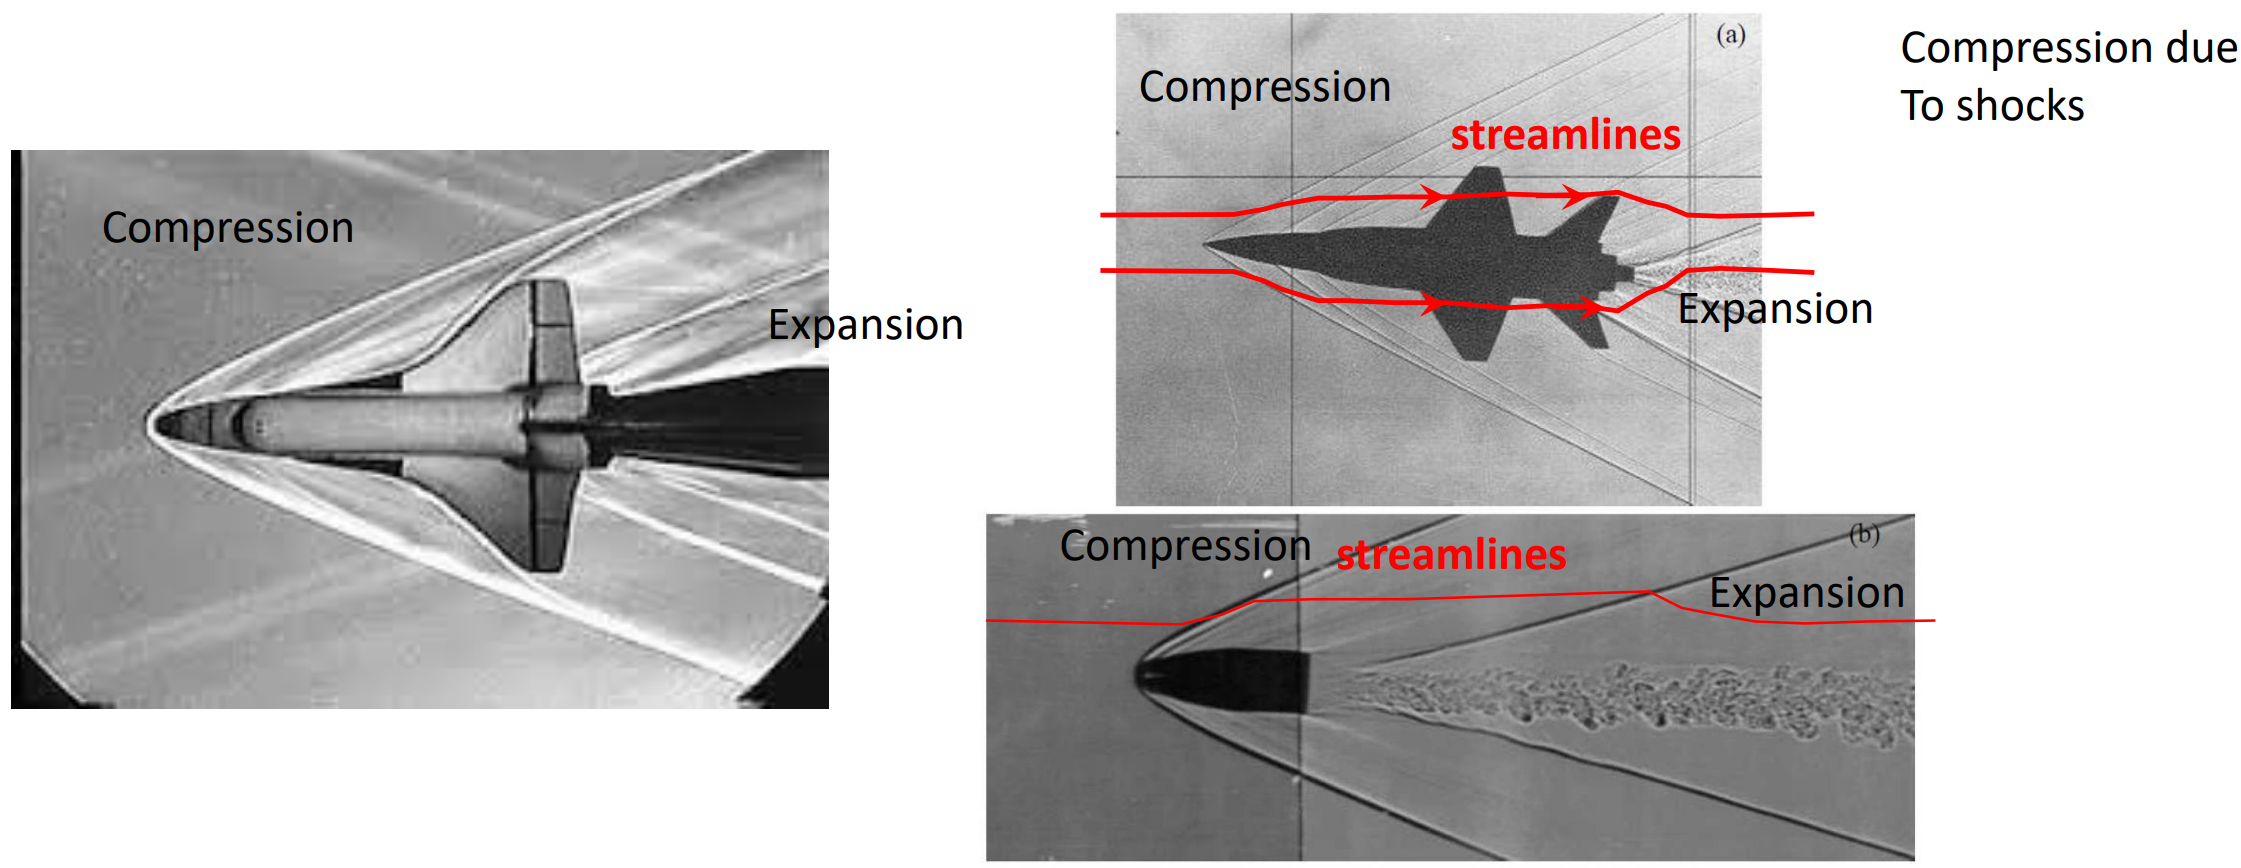
\includegraphics[width = \textwidth]{../img/diagram18.png}
    \caption{Examples of supersonic expansion.}
\end{figure}
\subsection{Sonic waves}
\begin{figure}[H]
    \centering
    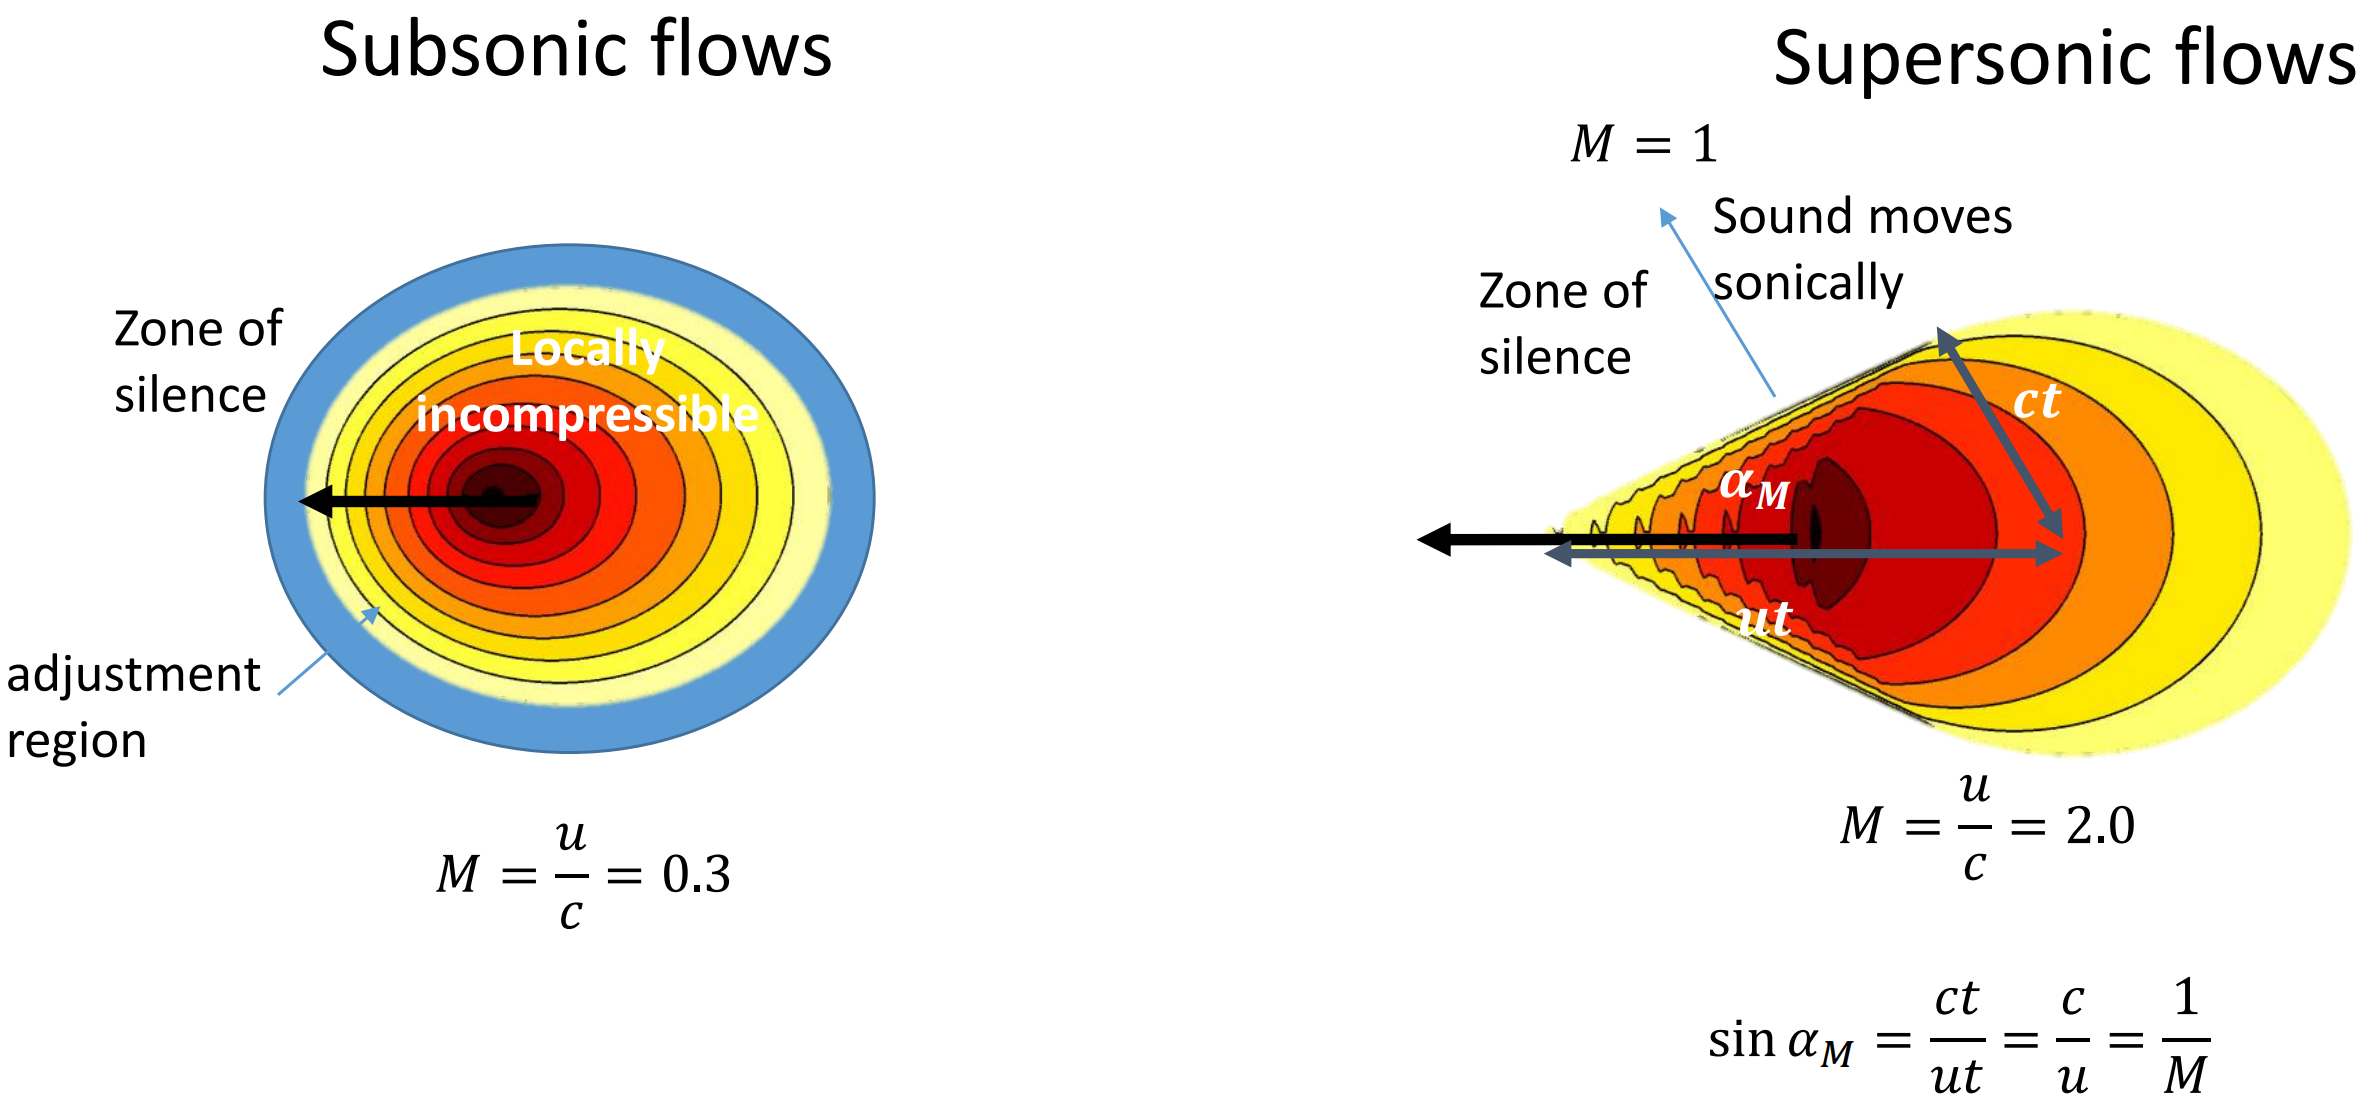
\includegraphics[width = \textwidth]{../img/diagram19.png}
    \caption{Sonic waves.}
\end{figure}
\subsection{Turning a corner}
\begin{figure}[H]
    \centering
    \begin{minipage}{.5\textwidth}
        \centering
        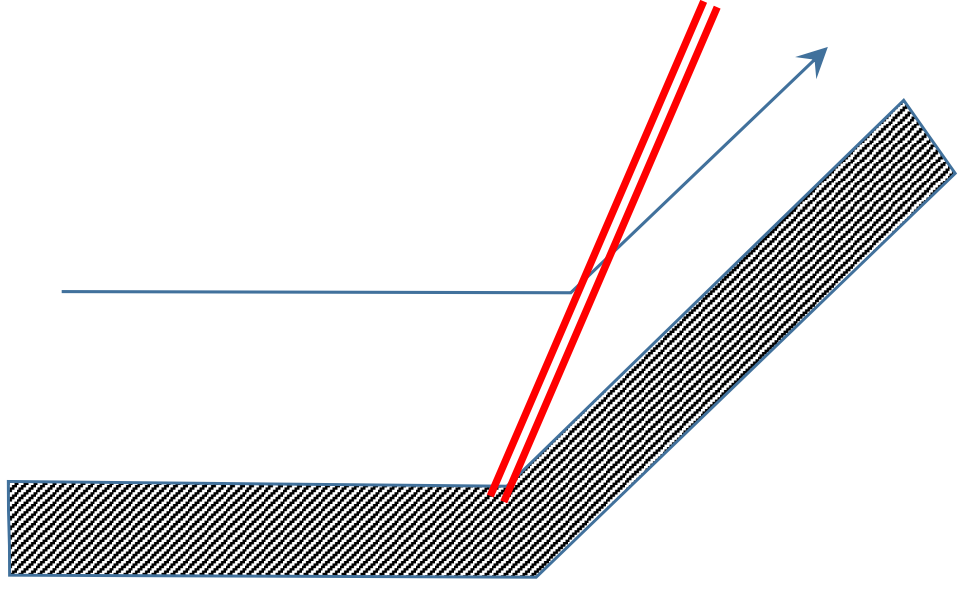
\includegraphics[width=.8\linewidth]{../img/diagram20.png}
        \captionof{figure}{Shock is formed. Entropy decreases.}
    \end{minipage}%
    \begin{minipage}{.5\textwidth}
        \centering
        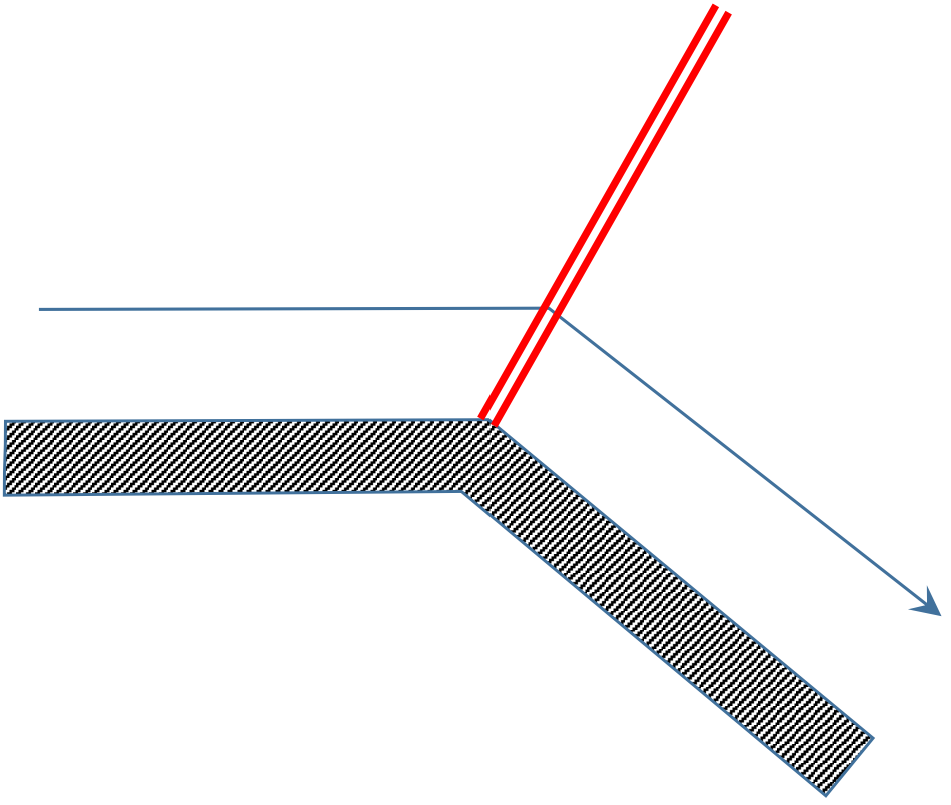
\includegraphics[width=.8\linewidth]{../img/diagram21.png}
        \captionof{figure}{If a single shock is formed, entropy increases and this is unphysical.}
    \end{minipage}
\end{figure}
A we have seen in the previous section, as the flow is turned by a wedge, the flow is compressed and the Mach number decreases. Whether the flow downstream of an oblique shock is supersonic depends on the deflection angle.
\begin{figure}[H]
    \centering
    \begin{minipage}{.5\textwidth}
        \centering
        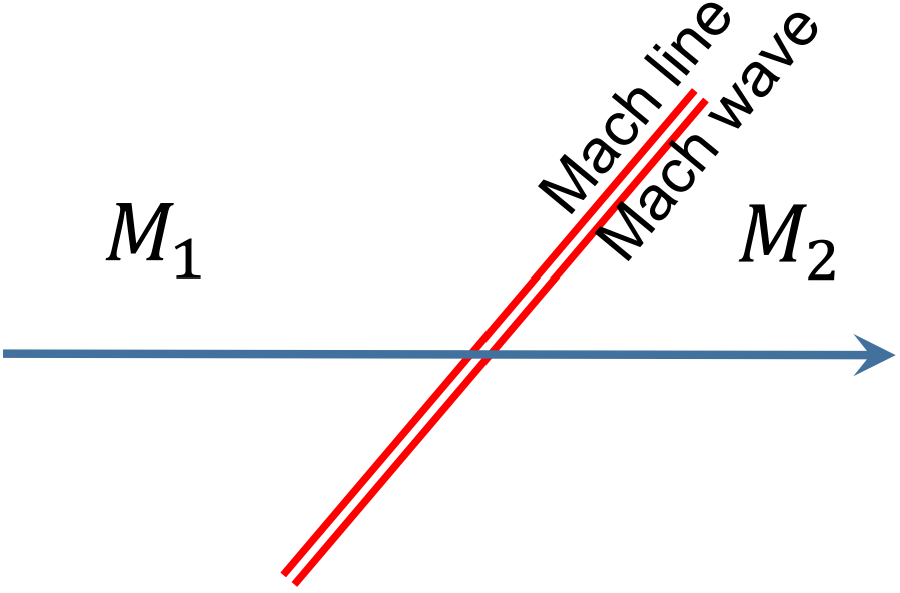
\includegraphics[width=.8\linewidth]{../img/diagram22.png}
        \captionof{figure}{}
    \end{minipage}%
    \begin{minipage}{.5\textwidth}
        \centering
        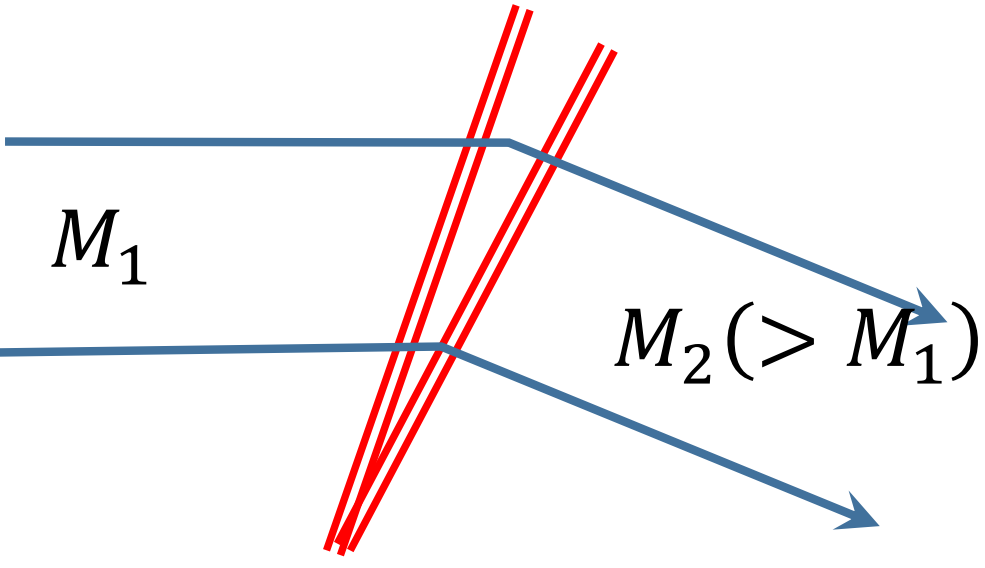
\includegraphics[width=.8\linewidth]{../img/diagram23.png}
        \captionof{figure}{}
    \end{minipage}
\end{figure}
A Mach line or waves is a very weak shock comprised of an isentropic process. We can study the relationship between the turning angle and the change in Mach number by studying the deflection process in more detail.

Here we consider the case where the flow expands and the process of adjustment. The Mach number of the flow will increase due to expansion, but the pressure wil decrease. The process of adjustment takes place by shockwaves being emitted. The first result we need to consider is the angle $\nu$ that the shock waves make to the incident flow.
\subsection{Schematic and notation}
\begin{figure}[H]
    \centering
    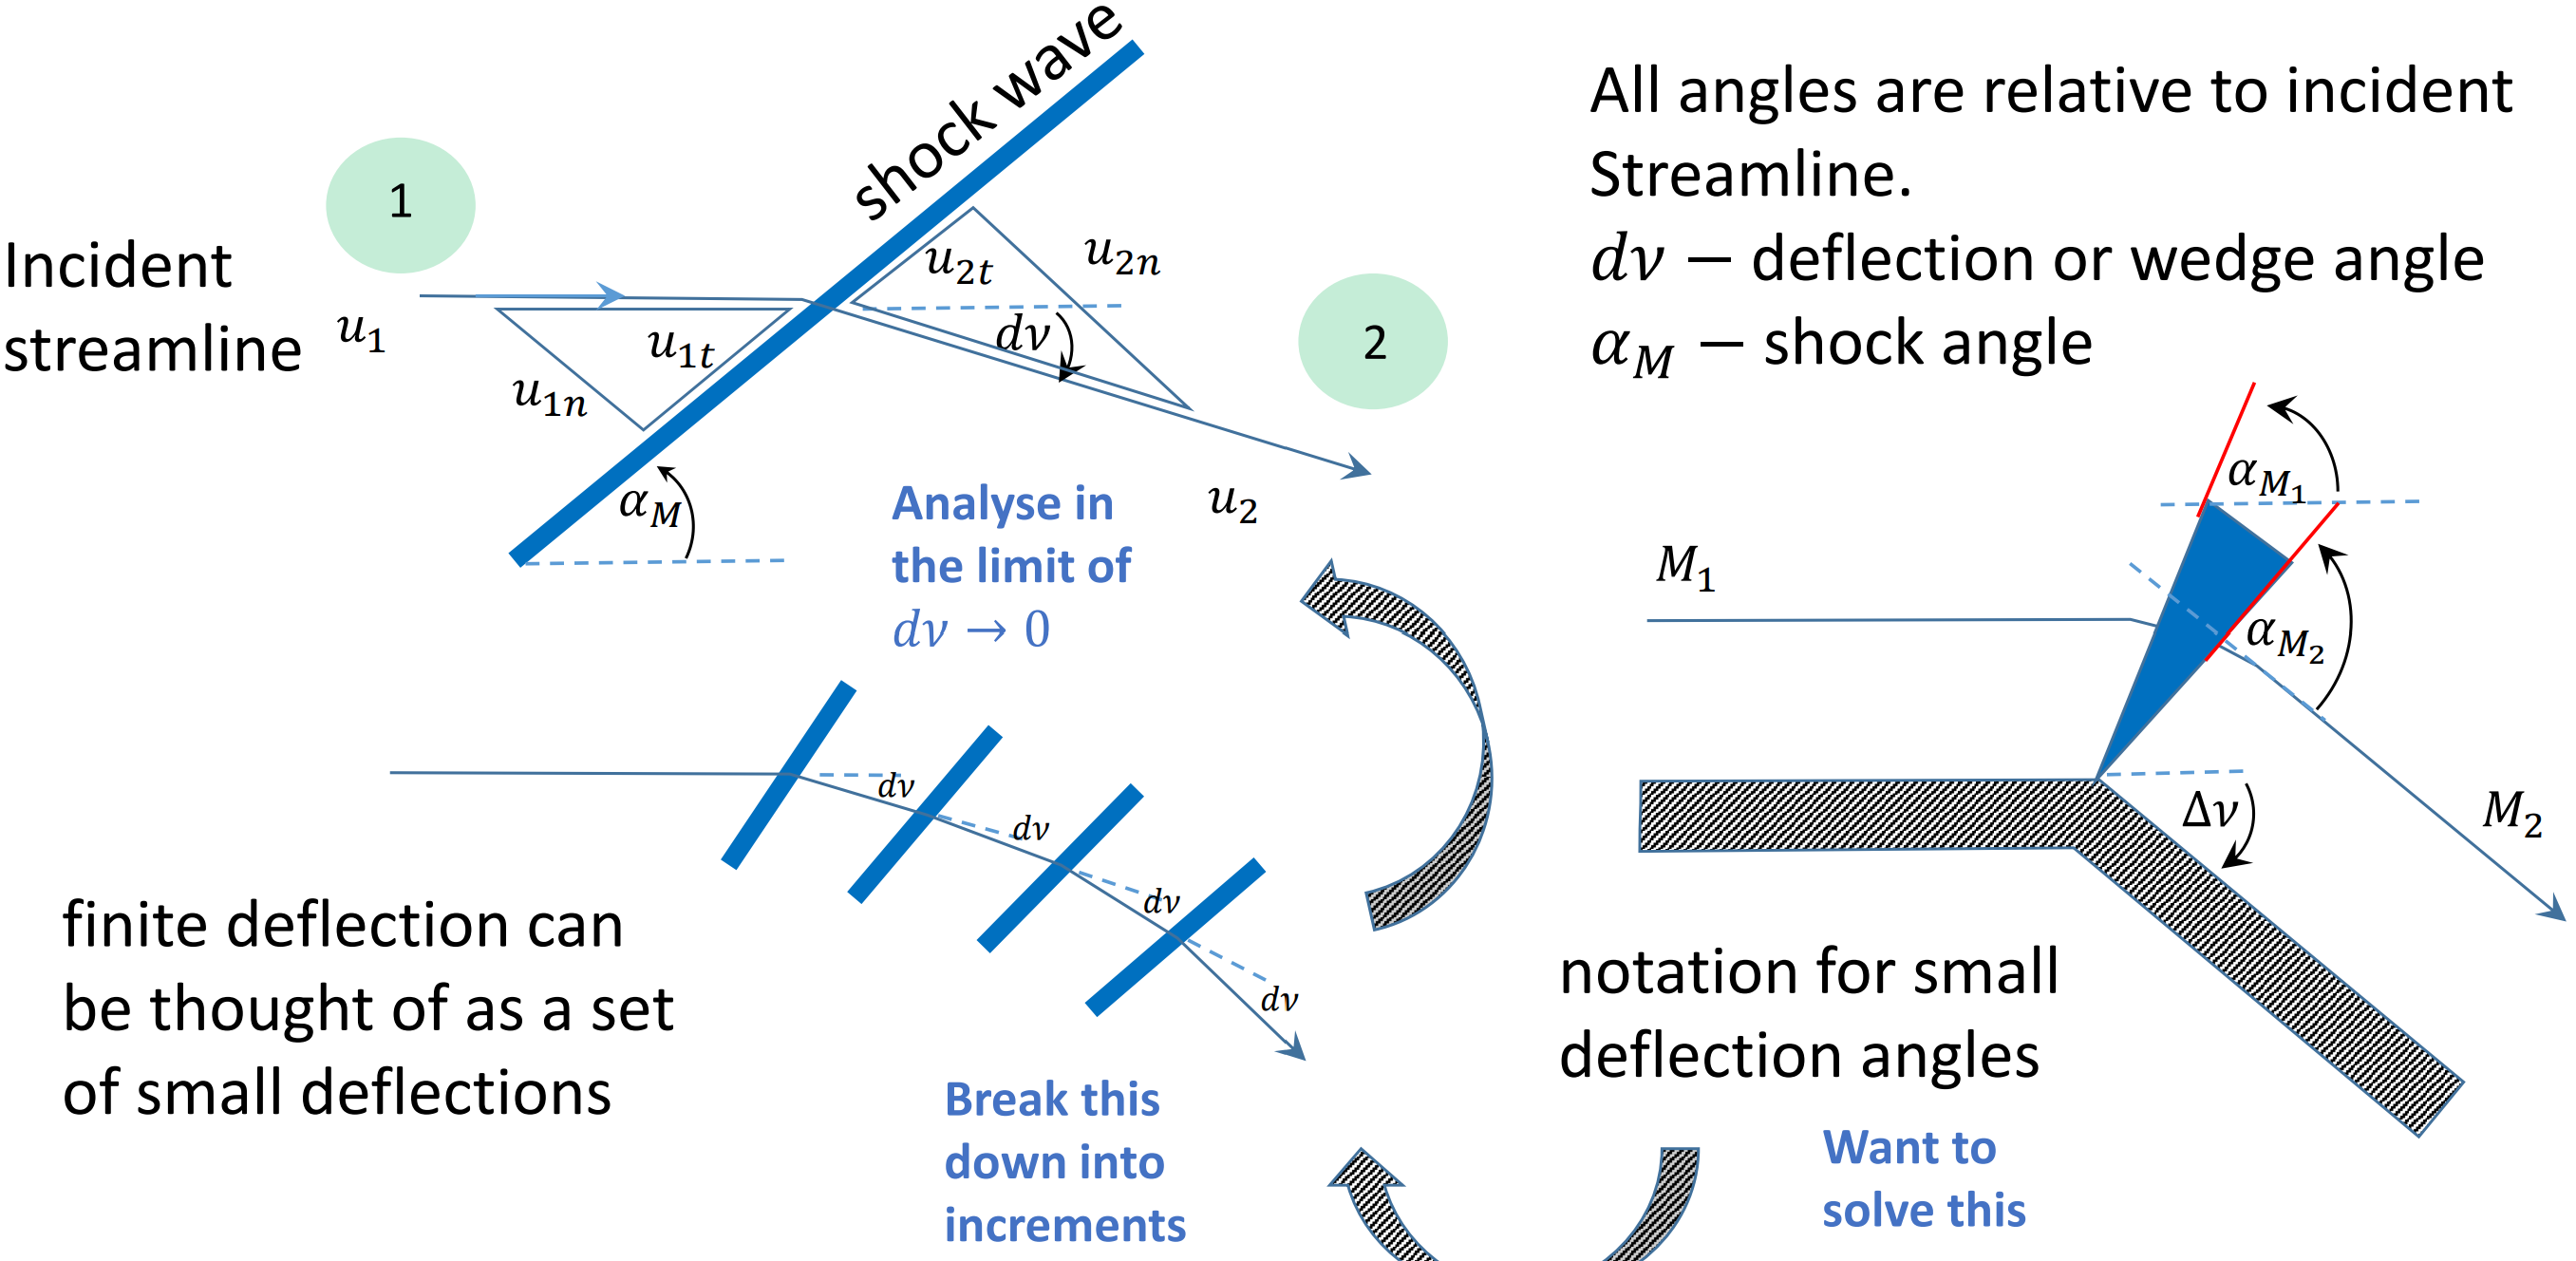
\includegraphics[width = \textwidth]{../img/diagram24.png}
    \caption{Schematic and notation.}
\end{figure}
\subsection{Geometrical characteristics}
The slip velocity is continuous so that:
\begin{equation}
    u_1 \cos \alpha_M = u_2 \cos\left(\alpha_M + \dif v\right)
\end{equation}
From the double angle formula:
\begin{equation}
    \cos \left(\alpha_M + \dif v \right) \approx \cos \alpha_M - \dif v \sin\alpha_M
\end{equation}
Rearranging gives:
\begin{equation}
    \frac{\dif u}{u} = \frac{u_2 - u_1}{u_2} = \frac{\sin\alpha_M}{\cos \alpha_M} \dif v
\end{equation}
Since the Mach wave angle $\alpha_m$ is related to the Mach number by:
\begin{equation}
    \sin\alpha_M = \frac{1}{M}
\end{equation}
Combining and using $\cos^2\alpha_M = 1 - \sin^2\alpha_M$, gives:
\begin{equation}
    \frac{\dif u }{u} = \frac{\sin \alpha_M}{\left(1 - \sin^2\alpha_M\right)^{\frac{1}{2}}}\dif v = \frac{\dif v}{\left(M^2 - 1\right)^{\frac{1}{2}}}
\end{equation}
We can write:
\begin{equation}
    \frac{u^2}{M^2} = \frac{u^2}{\left(\dfrac{u^2}{\gamma RT}\right)} = \gamma RT
\end{equation}
From the Conservation of Energy,
\begin{equation}
    T\left(1 + \frac{1}{2}\left(\gamma - 1\right)M^2\right) = \textrm{const}
\end{equation}
Taking the square root gives:
\begin{equation}
    \frac{u}{M}\left(1 + \frac{1}{2}\left(\gamma -1 \right)M^2\right)^{\frac{1}{2}} = \textrm{const}
\end{equation}
Taking the logarithm:
\begin{equation}
    \log u - \log M + \frac{1}{2}\log \left(1 + \frac{1}{2}\left(\gamma - 1\right)M^2\right) = \textrm{const}
\end{equation}
To find the differential change we take the differential to give us:
\begin{equation}
    \frac{\dif u}{u} - \frac{\dif M}{M} + \frac{\frac{1}{2}\left(\gamma - 1\right)\frac{1}{2}2M}{1 + \frac{1}{2}\left(\gamma - 1\right)M^2}\dif M = 0
\end{equation}
Rearranging gives:
\begin{align}
    \frac{\dif u}{u} & = \left(\frac{1}{M} - \frac{\frac{1}{2}\left(\gamma -1 \right)\frac{1}{2}2M}{1 + \frac{1}{2}\left(\gamma - 1\right)M^2}\right)\frac{\dif M}{M} \\
                     & = \frac{1}{1 + \frac{1}{2}\left(\gamma - 1\right)M^2}\frac{\dif M}{M}
\end{align}
Combining the above equations:
\begin{equation}
    \frac{\dif v}{\left(M^2 - 1\right)^{\frac{1}{2}}} = \frac{\dif u}{u} = \frac{\dif M}{M\left(1 + \frac{1}{2}\left(\gamma -1\right)M^2\right)}
\end{equation}
In total,
\begin{equation}
    \Delta v = \int_0^{\Delta v} = \int_{M_1}^{M_2} \left(\frac{\left(M^2 - 1\right)^{\frac{1}{2}}}{M \left(1 + \frac{1}{2}\left(\gamma - 1\right)M^2\right)}\right)\dif M
\end{equation}
\subsection{Relationship between turning angle and $M$}
\begin{equation}
    \Delta v = \int_0^{\Delta v} = \int_{M_1}^{M_2} \left(\frac{\left(M^2 - 1\right)^{\frac{1}{2}}}{M \left(1 + \frac{1}{2}\left(\gamma - 1\right)M^2\right)}\right)\dif M
\end{equation}
This is quite difficult to use since it would require tabulating $\Delta v$ against $M_1$ and $M_2$. Instead, we use the sonic reference condition and set $M_1 = 1$ and $M_2 = M$. This gives:
\begin{equation}
    v = \left(\frac{\gamma + 1}{\gamma -1}\right)^{\frac{1}{2}}\arctan\left(\left(\frac{\gamma + 1}{\gamma - 1}\right)^{\frac{1}{2}}\left(M^2 - 1\right)^{\frac{1}{2}}\right)-\arctan\left(M^2 - 1\right)^{\frac{1}{2}}
\end{equation}
This formula is plotted in the Prandtl-Meyer charts below.
\begin{figure}[H]
    \centering
    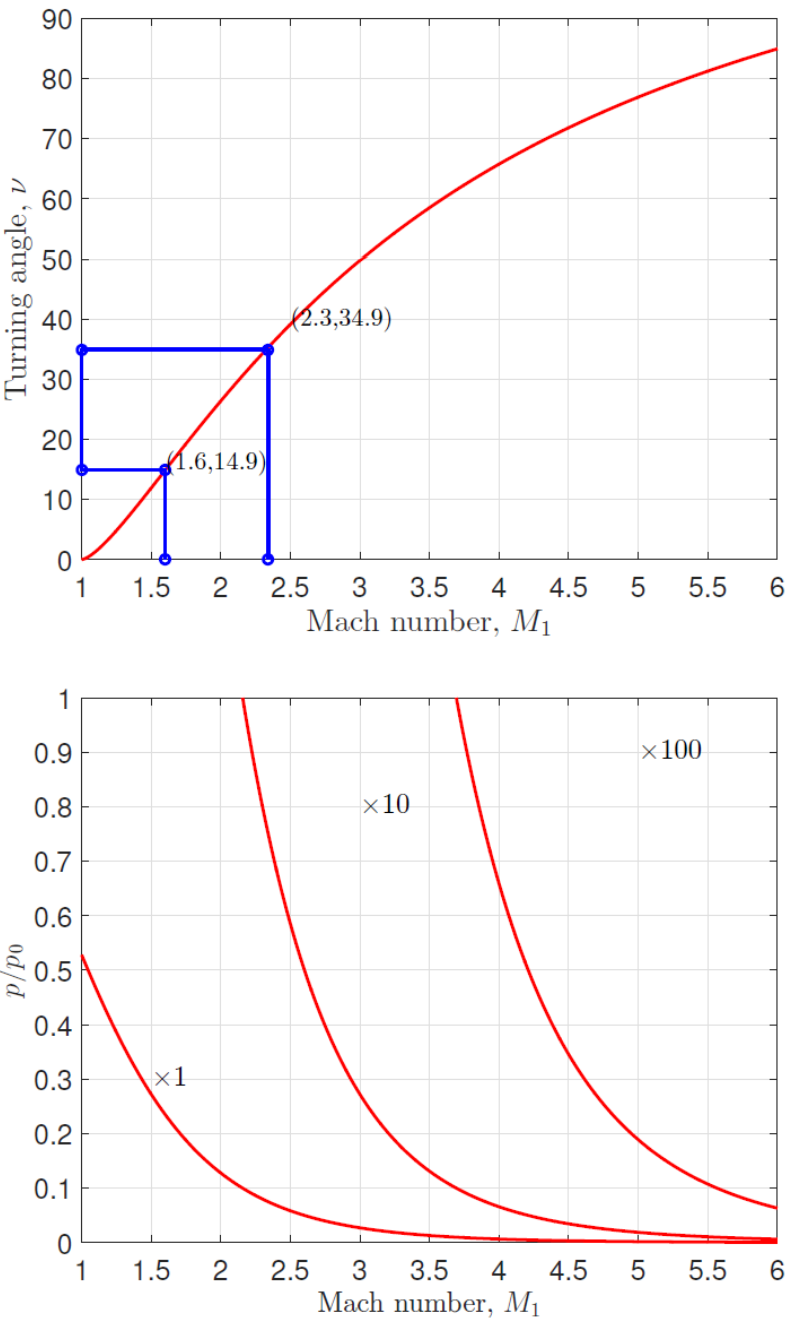
\includegraphics[width = 0.7\textwidth]{../img/diagram25.png}
    \caption{Prandtl-Meyer charts.}
\end{figure}
\subsection{How to use expansion charts}
\begin{figure}[H]
    \centering
    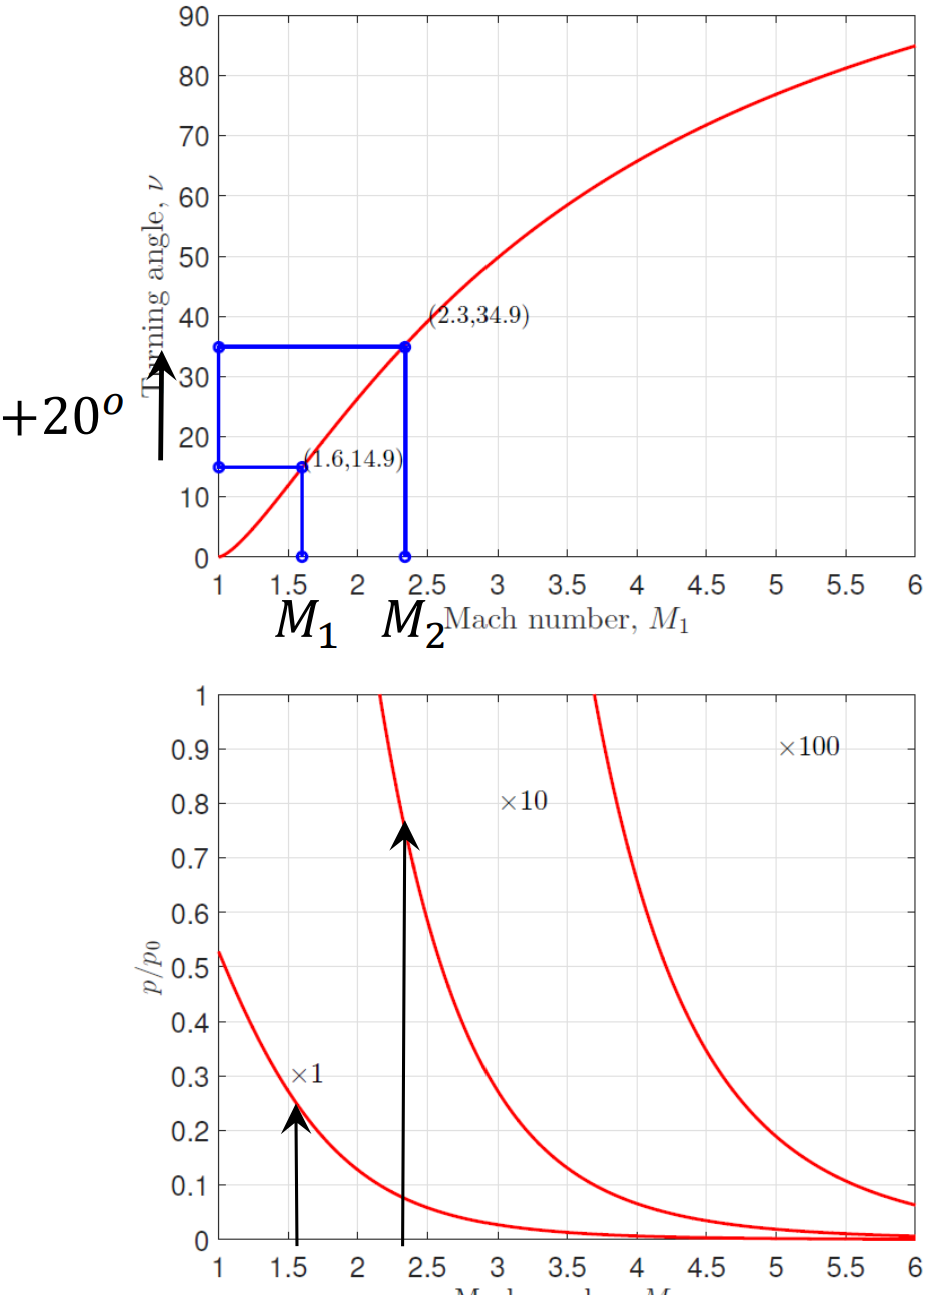
\includegraphics[width = 0.7\textwidth]{../img/diagram26.png}
    \caption{Prandtl-Meyer charts.}
\end{figure}
To illustrate how the charts are used, consider the finite deflection of a flow $M_1 = 1.6$ and the flow turns an angle $\Delta v = \SI{20}{\degree}$. We have to determine the turning angle from $M= 1$ to $M_1 = 1.6$. From the chart above this is $V_1 = \SI{14.9}{\degree}$. In total,
\begin{equation}
    v_2 = v_1 + \Delta v = \SI{14.9}{\degree} + \SI{20}{\degree} = \SI{34.9}{\degree}
\end{equation}
The corresponding Mach number is:
\begin{equation}
    M_2 = 2.31
\end{equation}
The fan angles are:
\begin{align}
    \alpha_{M_1} = \arcsin \frac{1}{M_1} = \SI{38.7}{\degree} \\
    \alpha_{M_2} = \arcsin \frac{1}{M_2} = \SI{25.7}{\degree}
\end{align}
For an expansion wave, the stagnation pressure is conserved.
\begin{align}
    p_0 & = p_1 \left(1 + \frac{1}{2}\left(\gamma - 1\right)M^2_1\right)^{\frac{\gamma}{\gamma -1}}  \\
        & = p_2 \left(1 + \frac{1}{2}\left(\gamma - 1\right)M^2_2\right)^{\frac{\gamma}{\gamma - 1}}
\end{align}
This enable the pressure after the expansion fan to be estimated. The stagnation pressure $p_0$ is constant across the expansion fan.
\subsection{Maximum turning angle}
\begin{figure}[H]
    \centering
    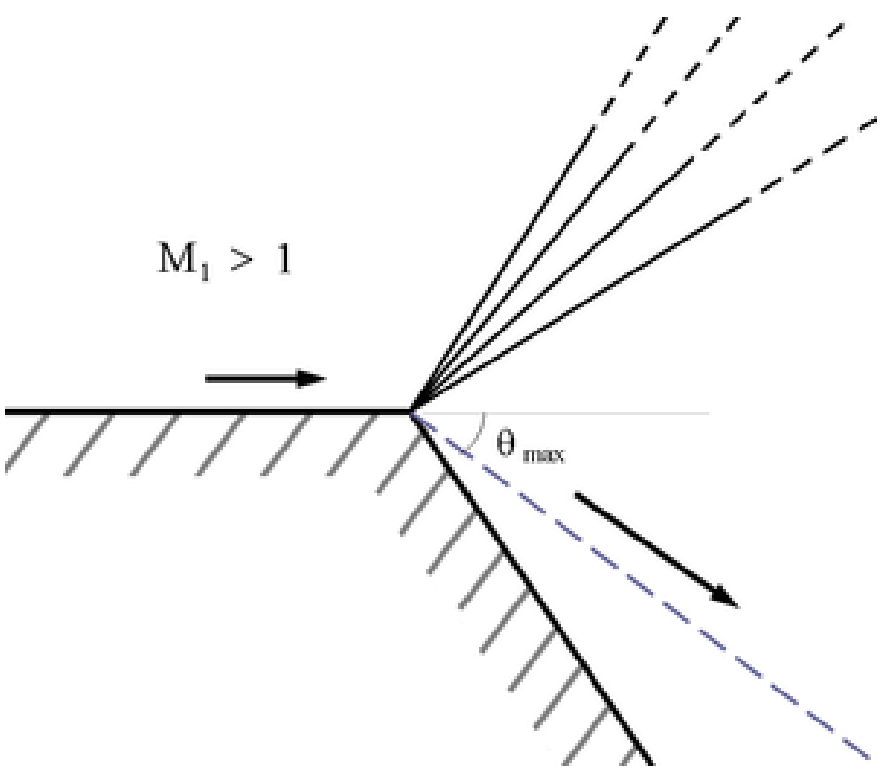
\includegraphics[width = 0.5\textwidth]{../img/diagram27.png}
    \caption{Prandtl-Meyer charts.}
\end{figure}
From the formula, we find that:
\begin{equation}
    v_{max} = \frac{\pi}{2}\left(\left(\frac{\gamma + 1}{\gamma -1}\right)^{\frac{1}{2}} - 1\right)
\end{equation}
This places a limit on the maximum turning angle that can be supported. When the deflection angle is greater than:
\begin{equation}
    \theta_{max} = v_{max} - v\left(M_1\right)
\end{equation}
a slip plane is generated.
\subsection{Turning a corner}
\begin{figure}[H]
    \centering
    \begin{minipage}{.5\textwidth}
        \centering
        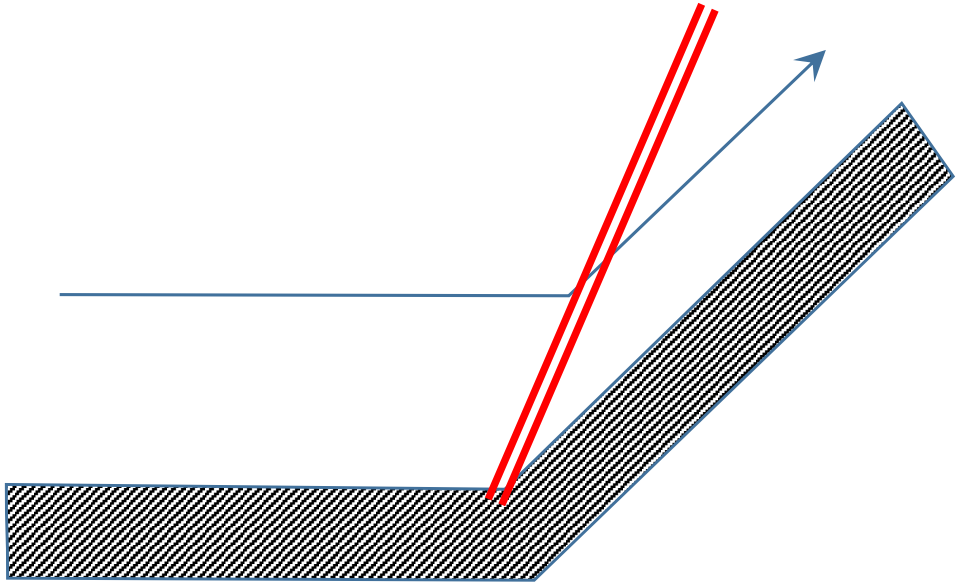
\includegraphics[width=.8\linewidth]{../img/diagram28.png}
        \captionof{figure}{Shock is formed.}
    \end{minipage}%
    \begin{minipage}{.5\textwidth}
        \centering
        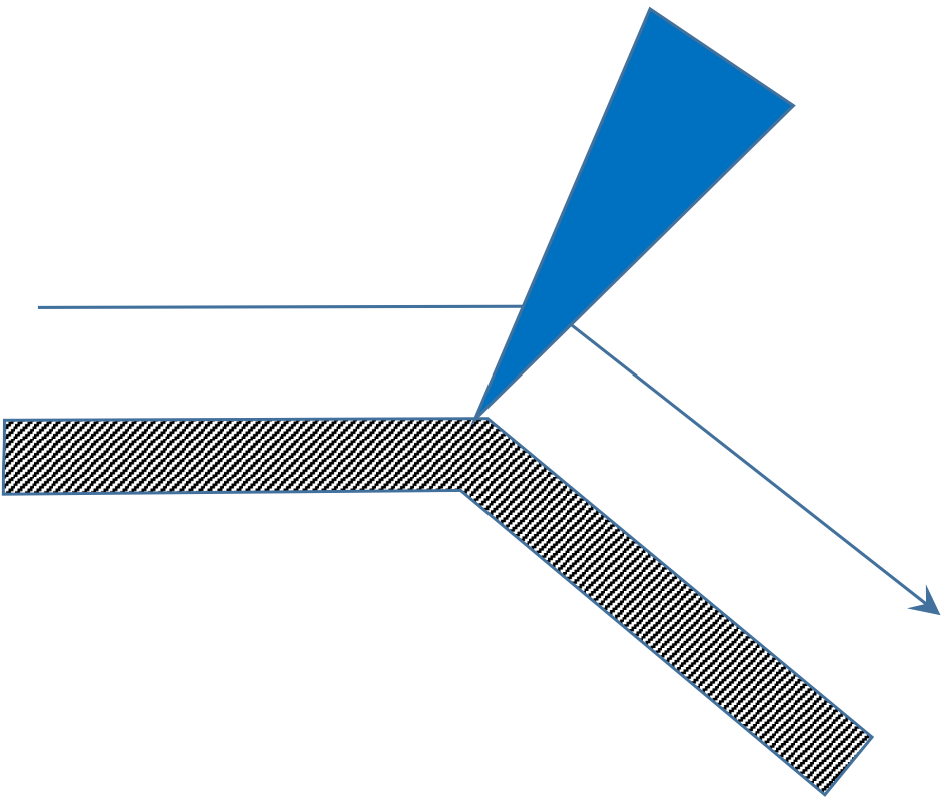
\includegraphics[width=.8\linewidth]{../img/diagram29.png}
        \captionof{figure}{Expansion fan.}
    \end{minipage}
\end{figure}
As we have seen in the previous section, as the flow is turned by a wedge, the flow is compressed and the Mach number decreases. Whether the flow downstream of an oblique shock is supersonic depends on the deflection angle.
\end{document}